\documentclass[tikz,border=8pt]{standalone}
\begin{document}
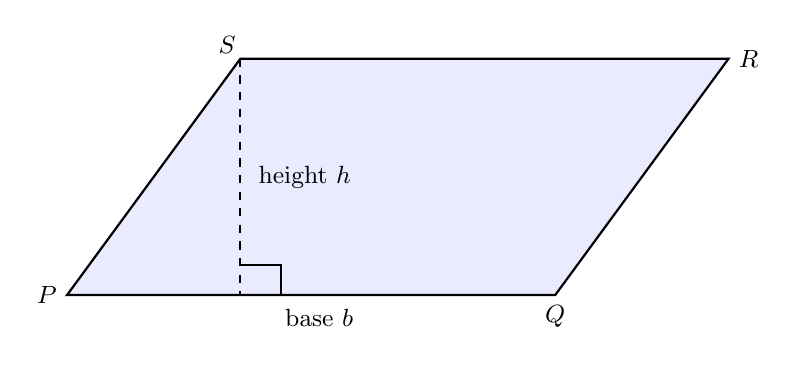
\begin{tikzpicture}[line width=0.8pt, font=\small]
  \coordinate (P) at (0,0);
  \coordinate (Q) at (6.2,0);
  \coordinate (R) at (8.4,3.0);
  \coordinate (S) at (2.2,3.0);
  \fill[blue!8] (P) -- (Q) -- (R) -- (S) -- cycle;
  \draw (P) -- (Q) -- (R) -- (S) -- cycle;
  \draw[dashed] (2.2,3.0) -- (2.2,0);
  \draw (2.2,0.38) -- (2.72,0.38) -- (2.72,0);
  \node[left] at (0,0) {$P$};
  \node[below] at (Q) {$Q$};
  \node[right] at (R) {$R$};
  \node[above left=-2pt] at (S) {$S$};
  \node[below] at (3.2,-0.05) {base $b$};
  \node[right] at (2.3,1.5) {height $h$};
\end{tikzpicture}
\end{document}
